\section*{Aquisição e Preparação}

Obtemos os dados para este trabalho prático de um \textit{Data Mart} da base de dados \newline\textit{`Adventure Works'} elaborado no primeiro trabalho prático. Este \textit{Data Mart} apresenta dados referentes a compras e vendas de uma empresa fictícia de bicicletas de nome igual à base de dados.

São ainda utilizados dois ficheiros \textbf{Excel} sobre dados de quantidade populacional e emissões de CO$_2$ de países, estes dados são proveninentes deste link:  \newline\text{\color{blue}{\url{https://data.worldbank.org/indicator?tab=featured}}}.  


\begin{figure}[H]
    \centering
    
    \tiny{
    \textcolor{blue}{\textbullet }{Dados sobre quantidade populacional}
    \textcolor{red}{\textbullet }{Dados sobre emissões de CO$_2$}
    }
    
    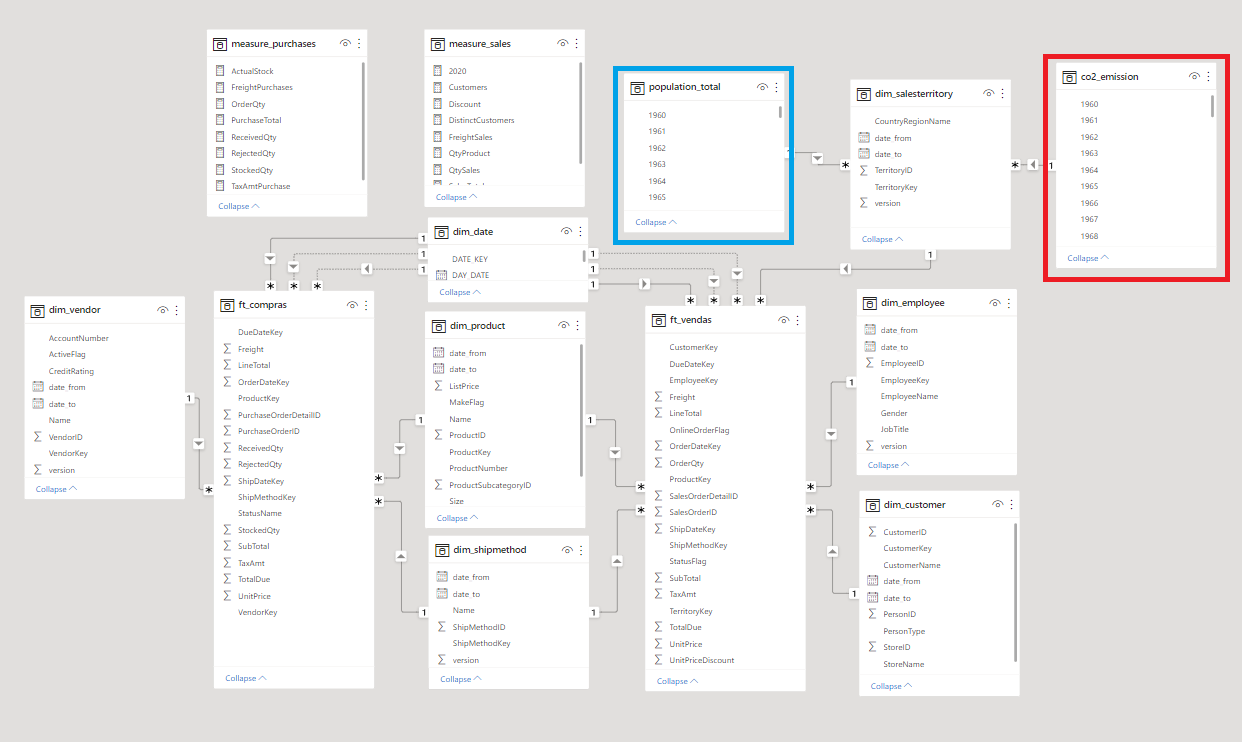
\includegraphics[scale=0.45]{images/DataMart.png}
    \selectlanguage{portuguese}\caption{Data mart utilizado}
    \label{fig:my_label}
\end{figure}

\subsection{Preparação dos dados Auxiliares (Excel)}

Dado o formato \textit{`human readable'} dos ficheiros transferidos, é necessário transformar os dados carregados utilizando a ferramenta \textit{Power Query}. Visto que ambos os ficheiros têm a mesma origem, estes seguem o mesmo formato sendo aplicável a ambos os seguintes procedimentos:

\begin{enumerate}
    \item Eliminação das 2 primeiras linhas.
    \begin{table}[H]
        \centering
        \begin{tabular}{|c|c|c|c|}
        \hline
            Last Updated Date & 16/12/2021 & \textit{null} & (...) \\
        \hline
            \textit{null} & \textit{null} & \textit{null} & etc.\\
        \hline
        \end{tabular}
    \end{table}
    
    \item Definição da (nova) primeira linha como Nome das Colunas
    \begin{table}[H]
        \centering
        \begin{tabular}{|c|c|c|c|}
        \hline
            Country Name & Country Code & Indicator Name & (...) \\
        \hline
        \end{tabular}
    \end{table}
\end{enumerate}